\documentclass[journal,10pt]{IEEEtran}
\usepackage{amsmath}
\usepackage{graphicx}
\usepackage{float}
\usepackage{comment}
\title{ \begin{huge}
\textbf{L2 Design Feasibility Report: Electric Skateboard} 
\end{huge} }
\begin{document}
\maketitle
\section{Executive Summary}
        This project consists of the design and construction of an electric skateboard based on a traditional longboard.
    
\section{Introduction}
        The scope of this project consists of designing an electric skateboard capable of carrying a large male on a round trip from the Josephine Butler College area to the Science Site and back via South Rd. The board's range should significantly exceed this base requirement in order to facilitate wider use. A longboard was supplied which will be modified non-invasively to produce the final product. 
\section{Board}
    \subsection{Overview}
        The board provided was a 'Raider I model (34’’ x 8’’)’ by Mindless Longboards [reference]. The deck was modelled in SOLIDWORKS and assembled with a downloaded model of the trucks [reference] - this allowed a FEA to be performed, to estimate locations and values of the max shear stress. Additionally, the strain and displacement profiles of the board under load were obtained. Material properties were taken for maple wood, as it is a common type of hardwood that is used for skateboard decks [reference].
    \subsection{Component Arrangements}
        Several arrangement options for the electrical components were explored, as shown in the figures below, with limiting factors consisting of:
        \begin{itemize}
            	\item Ground Clearance
            	\item Transmission Efficiency
            	\item Balance 
            	\item Rider Comfort
            \end{itemize}
        \begin{figure}[H]
                \centering
                \scalebox{0.25}{\includegraphics{"FEASIBILITY STUDY/Board/Concept_A".png}}
                \caption{Concept A
                \\*Deck clear
                \\*Motor close to driven wheel - efficient power transfer
                \\*Reduced ground clearance}
                \label{fig:ConceptA}
            \end{figure} 
        \begin{figure}[H]
                \centering
                \scalebox{0.15}{\includegraphics{"FEASIBILITY STUDY/Board/Concept_B".png}}
                \caption{Concept B
                \\*Maximum ground clearance, low transmission as components close to driven wheel
                \\*Board unbalanced (tail-heavy)
                \\*Component position detrimental to user comfort}
                \label{fig:ConceptB}
            \end{figure}  
        \begin{figure}[H]
                \centering
                \scalebox{0.15}{\includegraphics{"FEASIBILITY STUDY/Board/Concept_C".png}}
                \caption{Concept C
                \\*Maximum ground clearance
                \\*Components directly over front truck - no moment about front truck
                \\*Head-heavy - prevents board from tipping up
                \\*Components far from driven wheels - increased power losses
                \\*Components susceptible to damage at front}
                \label{fig:ConceptC}
            \end{figure} 
        \begin{figure}[H]
                \centering
                \scalebox{0.15}{\includegraphics{"FEASIBILITY STUDY/Board/Concept_D".png}}
                \caption{Concept D
                \\*Well-balanced
                \\*Motor close to driven wheel - efficient power transmission
                \\*Increased rider comfort - deck clear
                \\*Battery and motor separated - extensive cabling required
                \\*Separate casings required}
                \label{Fig:ConceptD}
            \end{figure} 
        \begin{figure}[H]
                \centering
                \scalebox{0.15}{\includegraphics{"FEASIBILITY STUDY/Board/Concept_E".png}}
                \caption{Concept E
                \\*Deck clear
                \\*Well-balanced as components aligned with centroid of board
                \\*Battery and motor can be integrated into single casing
                \\*Poor ground clearance
                }
                \label{Fig:ConceptE}
            \end{figure}
        Eventually it was decided that the arrangement shown in concept A provided the optimal compromise between the four factors.
    \subsection{Structural Analysis}
        The rider's load was assumed to total 1100N, distributed over two 10cmx10cm square areas at appropriate positions on the board. An additional load of 80N was applied at the centre of the wheelbase on a similar square area to model the weight of the electrical components.The simulation computed the maximum Von-Mises stress to be approximately 31.69MPa, located at the joint between the truck and the board, as shown below in the figures below.
        \begin{figure}[H]
            \centering
            \scalebox{0.15}{\includegraphics{"FEASIBILITY STUDY/Board/Stress_Analysis_Top".png}}
            \caption{FEM Von Mises Stress Analysis of Top Surface of the Board
            }
            \label{fig:stressTop}
        \end{figure}
        \begin{figure}[H]
            \centering
            \scalebox{0.15}{\includegraphics{"FEASIBILITY STUDY/Board/Stress_Analysis_Bottom".png}}
            \caption{FEM Von Mises Stress Analysis of Bottom Surface of the Board
            }
            \label{fig:stressBottom}
        \end{figure}
        Comparing this to the yield strength of maple wood, approximately 65.5MPa, a Factor of Safety value of approximately 2.1 was calculated. A further simulation was performed with the rider's load scaled up by this FOS, and the load located at a single 10cmx10cm area at the centre of the wheelbase. The max displacement was calculated as approximately 18.19mm, shown in figure 8 below. 
        \begin{figure}[H]
                \centering
                \scalebox{0.15}{\includegraphics{"FEASIBILITY STUDY/Board/Displacement".png}}
                \caption{Displacement Contour of Board When Put Under Maximum Loading
                }
                \label{fig:Displacement}
            \end{figure}
        This with consideration of the original board height - 110mm, allows a minimum ground clearance of approximately 91.81mm - this was considered to be a suitable value as it allows for electrical components to have a max height of 45.9mm considering a FOS of 2.
    
\section{Powertrain}
    \subsection{Transmission}
        \subsubsection{Belt}
            Due to the elasticity of rubber belts, this option provides low noise and vibration, and allows for efficient power transmission. Furthermore, they require relatively low maintenance and have a long lifespan. 
        \subsubsection{Gearing}
            Having the output of the motor go directly into a gear arrangement/gear box would allow for a vast array of gear ratios - however, this would require strong gears to provide the required torque, and the large range of output speeds of DC motors may make large gear ratios unnecessary.
        \subsubsection{Chain}
            Using a chain drive is the most efficient way to transmit power amongst the options covered, with a typical efficiency of 98\%. [REFERENCE P80 mechanical power efficiency] However, high maintenance is required due to the need for lubrication to prevent wear and corrosion. 
        \begin{figure}[H]
            \centering
            \scalebox{0.12}{\includegraphics{"./Drivetrain/Images/Drivetrain1Lab".png}}
            \caption{Arrangement with gears}
            \label{fig:Drivetrain1}
        \end{figure}
        \begin{figure}[H]
            \centering
            \scalebox{0.12}{\includegraphics{"./Drivetrain/Images/Drivetrain2Lab".png}}
            \caption{Arrangement with Belt/ Chain}
            \label{fig:Drivetrain2}
        \end{figure}
        \begin{figure}[H]
            \centering
            \scalebox{0.12}{\includegraphics{"./Drivetrain/Images/Drivetrain3Lab".png}}
            \caption{Arrangement with Belt attached to trucks}
            \label{fig:Drivetrain3}
        \end{figure}
        \subsubsection{Hub Motor}
            Hub motors are entirely contained in the wheels of the skateboard, offering many advantages including quietness, low maintenance and sleek appearance.
            However as they have no gearing and are limited in terms of the space of the wheels, they provide less torque than a traditional drive. %\[cooling?, wheel customization, ride- thin polyurethane]
    \subsection{Motor}
        \subsubsection{Required Parameters}
        %\The main requirements of the motor are:
        \begin{itemize}
        	\item Size- the motor must fit under the board
        	\item Torque- There should be enough torque to accelerate uphill - 10Nm at the wheel [figure]
        	\item Speed- The $K_{v}$ motor parameter should be 
        	\item Power- XXX
        \end{itemize}
        \begin{gather*}
            F = F_{Rolling Resistance} + F_{Acceleration} + F_{Gravity}
            \\F_{Acceleration} = Weight \times Gravity
            \\F_{Gravity} = Weight \times sin(Slope  Angle)
            \\F_{Rolling Resistance} = XXX value in wheels part
            \\Torque = F \times R_{Wheels}
            \\Wheel RPM = 
        \end{gather*}

        \subsubsection{AC Motor}
            The AC induction motor is the most common type of motor in large industrial applications due to its efficiency, reliability and durability. However, using a DC battery source would require a variable frequency inverter to produce an AC output to the motor and to control the speed, and particularly with single phase induction motors the staring toque is very low, which is unsuitable for this application. 
        \subsubsection{DC Brushed Motor}
            Using a commutator allows a motor to be run from a DC supply but by using carbon brushes adds a large amount of friction to the operation and varying the speed of this type of motor is harder, especially if two motors were implemented and required to run synchronously.
        \subsubsection{DC Brushless Motor}
            With an electronic speed control a motor can be run from a DC supply with simple control of speed. Also as this eliminates the need for a commutator there is less friction so greater efficiency, longer lifespan and reduced wight for the same output power. This motor family also gives a large staring torque so the board will be able to accelerate quickly at low speeds XXX. For these reasons it was decided a DC brushless motor would be used.
    \subsection{Battery}
        \subsubsection{Capacity}
            The greater the capacity of a battery network, the heavier and more expensive it becomes.The two main considerations regarding the required capacity are range and efficiency. The range will be determined by average daily usage (a 15.km round trip between Butler and Science site) and expected charge frequency (assumed to be once a week).
            \begin{figure}[H]
                \centering
                \scalebox{0.5}{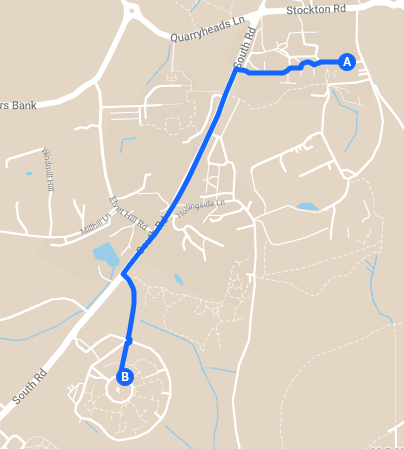
\includegraphics{./Battery/RouteAnalysis/Route.png}}
                \caption{Typical Daily Route}
                \label{fig:route}
            \end{figure}
            The elevation and gradient variations can be seen in the graphs below, with data sourced from XXXX GPS public database XXXX
            \begin{figure}[H]
                \centering
                \scalebox{0.5}{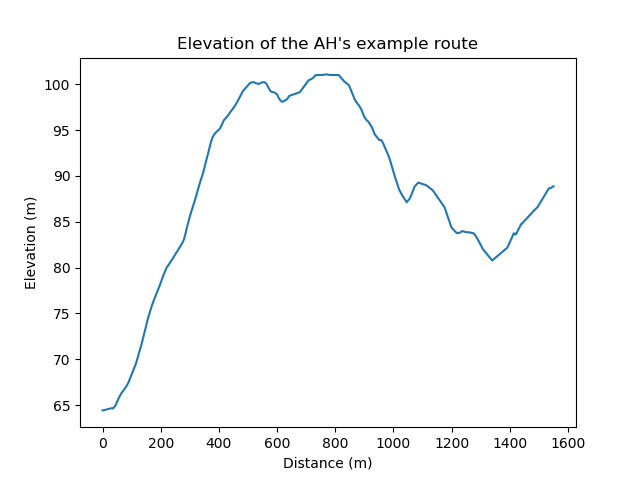
\includegraphics{./Battery/RouteAnalysis/elevation.png}}
                \caption{Elevation of Route}
                \label{fig:elevation}
            \end{figure}
            \begin{figure}[H]
                \centering
                \scalebox{0.5}{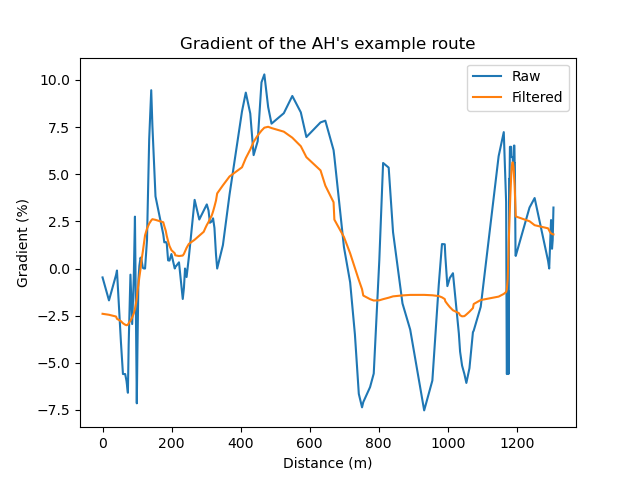
\includegraphics{./Battery/RouteAnalysis/grad.png}}
                \caption{Gradient of Route}
                \label{fig:gradient}
            \end{figure}
            The total elevation change consists of 50m uphill and 25m down (heading towards Josephine Butler). The energy required can be modelled as a simple vehicle hoist to give a rough estimate (Energy = $mg\Delta h$). The total vertical ascent over the trip is 75m, so we estimate that roughly 90kJ (25Wh) more energy will be required than with a perfectly efficient system.
        \subsubsection{Power Requirement Estimates}
            10Wh/mile (based off electric bike: 12Wh/mile)
            Total Power of Journey (including vertical): 37Wh
            Per Week Consumption: 5 x 37.5Wh = 185Wh
            -Absolute Minimum Required Capacity of 185Wh
        \subsubsection{Charging}
            Charging the battery is a complex concern, as specific charging circuits are required to prevent damage to the system. This is particularly true of modern batteries due to the large release of heat associated with large energy transfers.
        \subsubsection{Lifespan}
            The Lifespan of a battery is determined by the depth of discharge and the family of battery used.
            \begin{figure}[H]
                \centering
                \scalebox{0.5}{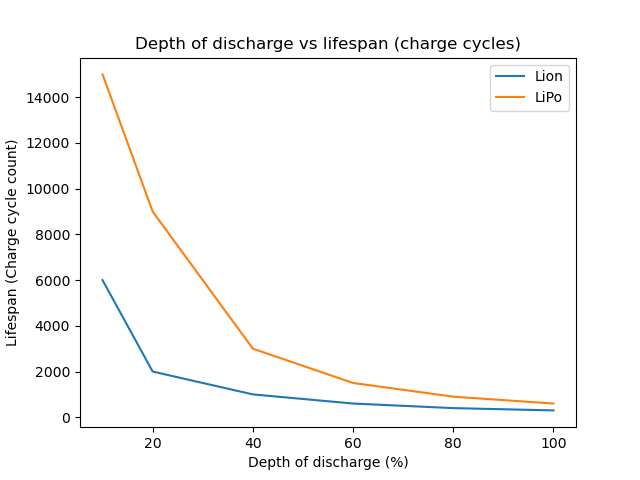
\includegraphics{./Battery/ChargeCycles/DoD.png}}
                \caption{Typical daily route}
                \label{fig:route}
            \end{figure}
            Lithium-ion batteries have a life cycle of approx. 800 cycles at 50\% DoD, whereas Lithium Polymer cells perform better at approx. 2000 charges at the same DoD - we will be using LiPo for this reason. Given that the capacity required at 100\% DoD is 185Wh, a 370Wh capacity is needed to achieve 50\% DoD.
        \subsubsection{Rate of Charge}
            As the rate of charge is a nonlinear function wrt. the charge level of the battery, the rate of recharge is specified from a DoD - general guidelines suggest that the charge rate should not exceed 1C to ensure optimal battery life.
        \subsubsection{Battery Size}
        Battery volume and weight are limiting factors wrt. capacity. Volume affects how the components can be arranged on the board, while weight directly impacts the board's performance.    
            \begin{figure}[H]
                \centering
                \scalebox{0.40}{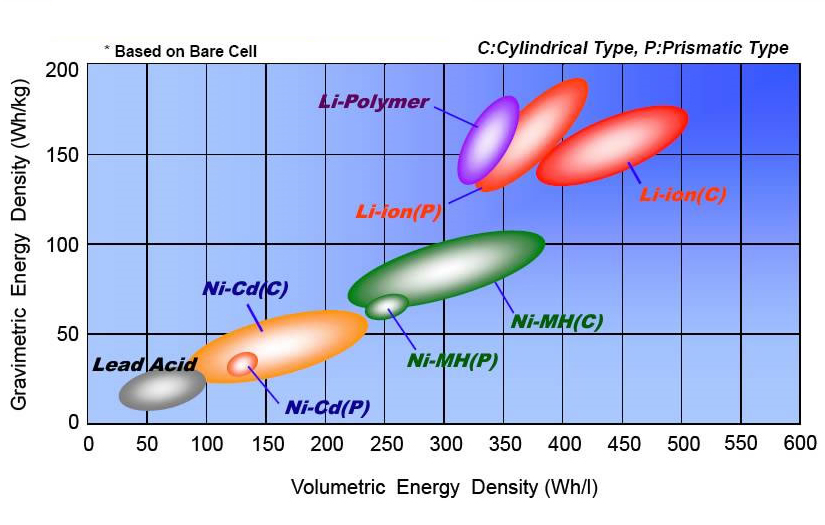
\includegraphics{./Battery/Density.png}}
                \caption{Credits: NASA - National Aeronautics and Space Administration}
                \label{fig:Battery Size}
            \end{figure}
\section{Trucks}
    \subsection{Operating Terrain}
        The board will be operating in an urban environment and will be running over mostly smooth surfaces - however, disturbances such as uneven patches of road, litter and debris will be present. As such, a suspension system is required to minimise the effects of such disturbances.
    \subsection{Speed Wobble}
        This phenomenon consists of unpredictable vibrations (approx. 4-10Hz) induced in the board when running at high speed – if neglected, these oscillations could directly affect the user’s ability to control the board, reducing user comfort and potentially resulting in injury. 
    \subsection{Potential Solutions}
        One option is to buy existing truck suspension systems- these would have the benefits of being pre-tested for similar operating requirements and freeing up development time. However, many of these are not the required dimensions, and lack important information and data sheets. Alternatively, numerical analysis of the requirements could allow us to design our own bespoke solution, and then consider its potential advantages compared to existing commercial suspension. 
\section{Wheels}
    \subsection{Overview}
        Many factors affect the choice of wheels – rolling resistance is affected by the wheel and bearings material, with the torque transferred dependent on the radii and material of the driven wheels.
    \subsection{Wheel Materials}
        Longboard wheels are typically made from polyurethane, which achieve a $\mu$-rolling in the range 0.04-0.08. While this is sufficiently small to provide low rolling resistance, polyurethane also only provides a $\mu$-static of ~0.2, limiting the torque that can be transferred to the road surface. This can be improved by using rubber for the driven wheels as rubber achieves a $\mu$-static in the range of 0.35-0.45, providing an increase in torque transmitted of 75-125\%.
    \subsection{Bearing Materials}
        Longboard bearings come in three different material families: steel, titanium and ceramic. Ceramic (Silicon Nitride) has a Brinell hardness 1479 kg/mm2, an increase of approx. 640\% over that of AISI-52100 steel and ASTM-7 Titanium, leading to reduced energy loss from elastic deformation. However, Silicon Nitride exhibits a yield strength of 170MPa: approx. 64\% less than steel and titanium. Ceramic may thus be inadvisable as the board will be used in an environment where it is expected to suffer shocks. Additionally, ceramic bearings cost significantly more than steel and titanium, the former often in the \$90-\$150 range, as opposed to \$15-\$20 and \$30 for steel and titanium respectively. Due to the similar properties of steel and titanium bearings, the latter’s corrosion resistance may suggest that it is the optimal type, less maintenance will be required. 
    \subsection{Wheel Dimensions}
        Longboard wheels typically vary in diameter between 60-100mm with a contact-patch width of approx. 30mm – larger wheel radii provide greater top speed and smoother ride, with smaller radii producing greater torque conversions. Depending on the output of the motor and the required road-torque, the appropriate wheel size can be selected.
    \subsection{Estimates of Rolling Resistance}
        \begin{figure}[H]
            \centering
            \scalebox{0.4}{\includegraphics{"FEASIBILITY STUDY/Wheels/Calculations_Diagram".png}}
            \caption{}
            \label{fig:Rolling Resistance Diagram}
        \end{figure}
    
    XXX[reference paper used]XXX
    
\section{Control}
    \subsection{Overview}
    	Any complex electronic system will almost always require a control unit to operate it.
    	There are three aspects of control that must be designed for; the user interface to control the skateboard, battery management, and motor/drive train control.
    	For this application, and the one-off nature of the product, it would be most effective to use a micro-controller system on a chip for control, rather than a bespoke hardware solution.
    	This is due to the ease of altering functionality, and the high volume of support documentation for these units.
    	Due to time and budget constraints, it would also be more effective to search for existing circuit modules than trying to design and build bespoke layouts.
    \subsection{User Interface}
        \begin{figure}[H]
            \centering
            \scalebox{0.2}{\includegraphics{"FEASIBILITY STUDY/Control/Boosted Remote Labelled".png}}
            \caption{Market Leader's Remote Control}
            \label{fig:Boosted Remote}
        \end{figure}
        \begin{figure}[H]
            \centering
            \scalebox{0.2}{\includegraphics{"FEASIBILITY STUDY/Control/Pressure Pads
            Labelled".png}}
            \caption{Dual Pressure Pad Control}
            \label{fig:Pressure Pads}
        \end{figure}
            
    	\subsubsection{Throttle Control}
    		The user needs to be able to control the speed of the board intuitively and quickly, to ensure safe riding.
    		The market leader utilises wireless controller (as shown Fig \ref{fig:Boosted Remote}) allowing for braking, accelerating and reverse, with fine step-wise control for each by a roller potentiometer.
    		This only takes effect when a secondary button is held, acting as a dead-mans-switch.
    		A potential solution to this is a dual pressure pad system, pictured in Fig \ref{fig:Pressure Pads}.
            
    	\subsubsection{Status Meters}
    		The user needs to be able to understand the remaining range of the board, so that they know the remaining time available.
    		The current market leader uses an array of LEDs on its controller for status. This can easily be improved on using 7 segment displays or a small LCD, allowing for numerical data to be shown to the rider. (shown in Fig. \ref{fig:7 seg} and Fig.\ref{fig:LCD}).
    		
    	\begin{figure}[H]
            \centering
            \scalebox{0.4}{\includegraphics{"FEASIBILITY STUDY/Control/7 Segment Labelled".png}}
            \caption{7 Segment Displays}
            \label{fig:7 seg}
        \end{figure}
    	\begin{figure}[H]
            \centering
            \scalebox{0.4}{\includegraphics{"FEASIBILITY STUDY/Control/LCD Labelled".jpg}}
            \caption{Arduino LCD}
            \label{fig:LCD}
        \end{figure}
    \subsection{Battery Management}
    	Care must be taken to ensure that in normal operation the battery is not charged or discharged outside of safe conditions.
    	This includes tracking the number of cycles the battery has gone through, as well as temperature, with a view to stop the rider from using the system if the battery is no longer in a safe state.
    	
    		%General guidelines suggest charging at no faster than 1C for optimal battery lifetime, meaning a 1300maH battery is charged at 1.3A for a duration of 1 hour.
    		%Discharge ratings vary depending on the battery, a typical hobby grade battery used for multi-rotors and helicopters boast a continuous draw of 40-50C, with a 10s burst of 90-120C, much higher than the charging rating.
    		%The number of cycles must be counted, as well as the current battery temperature to ensure that the battery is in a healthy state whenever in use.
    		%This includes preventing charging when the battery has reached the end of its operational lifetime.
    		%If regenerative braking is pursued, the circuitry must be carefully controlled so that the charging current is not exceeding these values.
    \subsection{Motor Control}
    		Since a DC Brushless motor is being used, a more complex control method is required than a brushed DC motor.
    		This circuitry can be obtained off the shelf as an 'Electronic Speed Controller' and are widely available in a range of specifications due to their use in the remote control model industry.
    		Control of these circuits is by pulse width modulation, or serial interface, varying by model and age of controller, signals that can be generated simply with a microcontroller.
    		This circuit could be designed and produced by hand, however due to the complexity, and the competitive pricing of the currently available products, it may prove a more effective choice to purchase an existing ESC.
    	%\subsection{Feedback}
    		%text goes here
\section{Conclusion}
From our research, a number of design conclusions have been drawn: a chain-drive and brushless DC motor were selected due to their optimal efficiency, while rubber wheels were settled on for the driven axle due their improved grip over polyurethane. Titanium bearings offer a compromise between performance and durability, with the final component layout providing the optimal trade-off between efficiency, ground clearance and rider comfort.
\section{References}

\end{document}